\documentclass[12pt]{article}

\usepackage[utf8]{inputenc}
\usepackage[brazil]{babel}
\usepackage{amsmath,amssymb}
\usepackage{pdfsync}
\usepackage[all]{xy}
\usepackage{color}
\usepackage{algorithm}
\usepackage{algpseudocode}
\usepackage{graphicx}
\usepackage{listings}
\usepackage{lmodern}
\usepackage{float}

\lstset{
    basicstyle=
    \fontencoding{T1}
    \fontfamily{lmtt}
    \fontseries{lc}
    \selectfont
}

\newcommand{\HI}{\textit{h.i.}}


\title{{\large Universidade de Brasília \\ Instituto de Ciências Exatas \\
Departamento de Ciência da Computação} \\[1cm]
117536 - Projeto e Análise de Algoritmos Turma: B\\[.5cm]
Relatório sobre {\\ \bf Complexidade do Bubblesort}}
\author{Camila F. T. Pontes - 15/0156120 \\
        Diogo C. Ferreira - 11/0027931}
\date{\today}

\begin{document}
\maketitle

\section{Introdução}
\indent \indent O problema de ordenação de sequências numéricas surge frequentemente em aplicações computacionais. Este problema pode ser definido formalmente da seguinte maneira \cite{cormen2009introduction}:
\begin{itemize}
    \item \textbf{Entrada:} uma sequência de $n$ números, $a_1, a_2, ..., a_n$
    \item \textbf{Saída:} uma permutação (reordenação) da sequência de entrada, $a'_1, a'_2,...,a'_n$ tal que $a'_1 \leq a'_2 \leq ... \leq a'_n$ 
\end{itemize}

Existem diversos algoritmos de ordenação que resolvem o problema apresentado acima, \textit{e.g.} \textit{insertion sort}, \textit{selection sort}, \textit{merge sort}, \textit{quicksort}, dentre outros. Neste trabalho, vamos analisar um dos algoritmos de ordenação mais simples, o \textit{bubblesort}. A ideia geral do \textit{bubblesort} é percorrer diversas vezes o vetor de entrada e, a cada passagem, mover para o final da porção ainda não ordenada o maior elemento. Uma implementação recursiva desse algoritmo é apresentada a seguir (Algoritmo \ref{algo:bubblesort}).

\begin{algorithm}[!h]
    \begin{algorithmic}[1]
        \Function{bubblesort}{int array $A$, int $n$}
            \If{n = 1}
                \State \Return
            \EndIf
            \For{$i \leftarrow 1$ to $n-1$}
                \If{$A[i] > A[i+1]$}
                    \State swap($A[i], A[i+1]$)
                \EndIf
            \EndFor
            \State bubblesort($A$,$n-1$)
            
        
        \EndFunction
    \end{algorithmic}\vspace{-2pt}
    \caption{Implementação recursiva do \textit{bubblesort}}
    \label{algo:bubblesort}
\end{algorithm}

Uma das formas de comparar o desempenho do \textit{bubblesort} com o desempenho de outros algoritmos de ordenação é através de uma análise de complexidade.
A complexidade do \textit{bubblesort} é de ordem quadrática ($O(n^2)$), \textit{i.e.}, no pior caso, são feitas $n^2$ trocas durante a ordenação, onde $n$ é o número de elementos do vetor de entrada.
Neste trabalho, um assistente de prova será utilizado para provar a complexidade do \textit{bubblesort}. 
A prova será realizada utilizando o \textit{Prototype Verification System} (PVS) \cite{owre1992pvs}. \\

Os principais objetivos deste trabalho são:
\begin{itemize}
    \item Implementar uma versão recursiva do \textit{bubblesort} com um contador para o número de trocas realizadas durante a ordenação;
    \item Provar a complexidade assintótica do \textit{bubblesort} utilizando o PVS.
\end{itemize}

%Na próxima seção, será realizada uma apresentação detalhada do problema.

\section{Apresentação do Problema}
\subsubsection{Funções auxiliares}

Para a realização da análise assintótica do Bubblesort,
inicialmente foram definidas três funções auxiliares
com o objetivo de rastrear as contagens do número total
de comparações realizadas pelo algoritmo após retornar
a lista ordenada.

\begin{itemize}
\item \texttt{bubbling\_count}: recebe uma lista $l$, um
natural $n$ (equivalentes aos parâmetros da função
\texttt{bubbling} original) e um contador $count$, que é
incrementando quando alguma comparação for realizada.
Seu valor de retorno é o par $(l, count)$ com a lista e
o contador devidamente atualizados.
\item \texttt{bubblesort\_aux\_count}: recebe uma lista $l$,
um natural $n$ (equivalentes aos parâmetros da função
\texttt{bubblesort\_aux} original) e um contador $count$,
que é passado para a função \texttt{bubbling\_count}
chamada internamente. Seu valor de retorno é o par
$(l, count)$ com a lista e o contador devidamente
atualizados.
\item \texttt{bubblesort\_count}: recebe uma lista $l$,
um natural $n$, equivalentes aos parâmetros da função
\texttt{bubblesort} original. Ela chama
\texttt{bubblesort\_aux\_count} da mesma forma que
\texttt{bubblesort} chama \texttt{bubblesort\_aux},
mas com o parâmetro do contador iniciando em 0. Seu valor
de retorno é o par $(l, count)$ com a lista ordenada
e o contador atualizados com o número total de comparações
realizadas pelo algoritmo.
\end{itemize}

\subsubsection{Lemas}
Lemas utilizados na prova da complexidade de \texttt{bubbling\_count}:
\begin{itemize}
    \item \texttt{bubbling\_equiv}: atesta a equivalência entre \texttt{bubbling} e \texttt{bubbling\_count}
    \item \texttt{bubbling\_length}: afirma que a função \texttt{bubbling\_count} não altera o tamanho da lista de entrada
    \item \texttt{bubbling\_counts\_n}: afirma que \texttt{bubbling\_count} realiza exatamente $n$ comparações, onde $n$ é o tamanho da lista de entrada, e que, portanto, sua complexidade é linear
\end{itemize}
Lemas utilizados na prova da complexidade de \texttt{bubblesort\_aux\_count}:
\begin{itemize}
    \item \texttt{bubblesort\_aux\_equiv}: atesta a equivalência entre \texttt{bubblesort\_aux} e \texttt{bubblesort\_aux\_count}
    \item \texttt{bubblesort\_counts\_n2}: afirma que \texttt{bubblesort\_aux\_count} realiza exatamente $n(n+1)/2$ comparações, onde $n$ é o tamanho da lista de entrada, e que, portanto, sua complexidade é quadrática
\end{itemize}
Lemas utilizados na prova da complexidade de \texttt{bubblesort\_count}:
\begin{itemize}
    \item \texttt{bubblesort\_equiv}: atesta a equivalência entre \texttt{bubblesort} e \texttt{bubblesort\_count}
    \item \texttt{bubblesort\_counts\_n2}: afirma que \texttt{bubblesort\_count} realiza exatamente $n(n-1)/2$ comparações, onde $n$ é o tamanho da lista de entrada, e que, portanto, sua complexidade é linear
\end{itemize}



\subsubsection{\textit{Bubbling}}

\paragraph{Lema \ref{lemma:bcount}: \texttt{bubbling\_counts\_n}:} seja $l$ uma lista de números naturais, e lembrando
que \texttt{bubbling\_count} é uma função que retorna um par $(l,c)$, onde $c$ denota o número
de comparações realizadas ao todo na chamada
\begin{equation*}
    \forall_{l,n,c} bubbling\_count(l, c, n)_2 = c + n \hspace{1cm}, n<|l|, c\in \mathbb{N}
\end{equation*}

\paragraph{Estratégia da prova:} indução forte sobre $|l|$.
A função \texttt{bubbling\_count} faz chamadas recursivas sobre $l$, e seria
correspondente às linhas 5 a 9 do Algoritmo \ref{algo:bubblesort}.
Cada chamada é feita sobre uma lista menor mas a lista não é dividida
exatamente conforme a definição recursiva de $l$. Portanto precisamos de
uma medida alternativa que seja relacionada com a estrutura
sobre a qual queremos realizar a indução (Figura \ref{fig:bubbling1}).

\begin{figure}[h!]
    \centering
    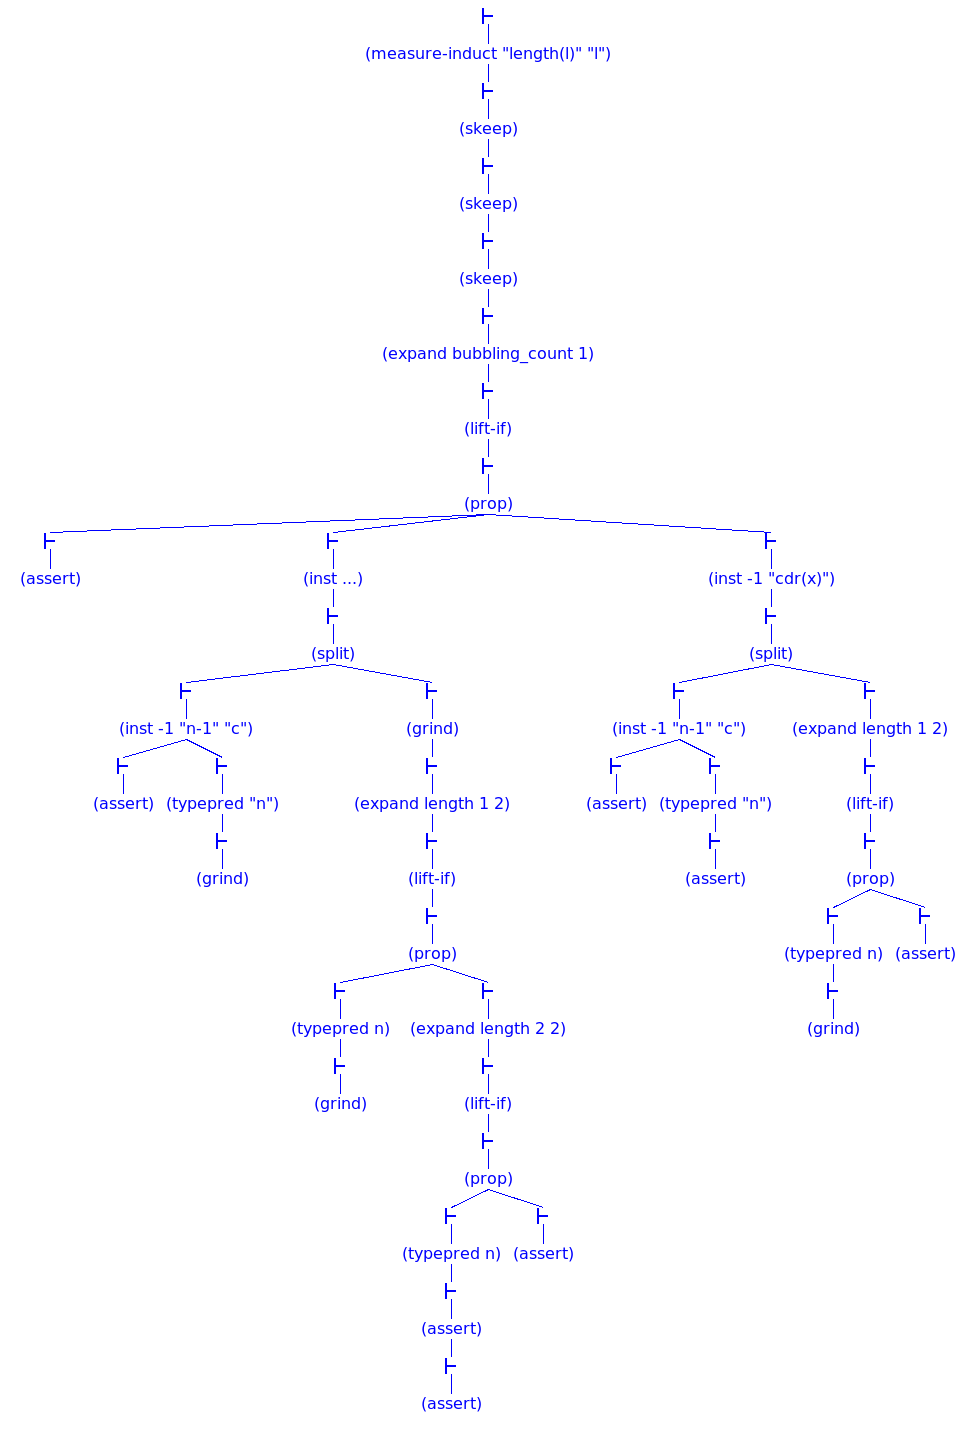
\includegraphics[width=0.5\linewidth,trim={8cm 35cm 8cm 0},clip]{figures/bubbling-counts-n.png}
    \caption{A prova do lema de complexidade de \texttt{bubbling\_count} foi realizada
    por indução forte sobre $|l|$.}
    \label{fig:bubbling1}
\end{figure}

Após a expansão da definição da definição de \texttt{bubbling\_count}, precisamos
provar 3 casos: o caso em que $n=0$ (trivial, pois $c = c + n = c + 0 = c$), 
o caso em que $l_i > l_{i+1}$ e o caso em que $l_i \leq l_{i+1}$. A prova destes dois
últimos casos é muito semelhante, e varia essencialmente em como a hipótese de indução
(\HI) será instanciada (Figura \ref{fig:bubbling2}). No primeiro caso,
a próxima chamada de \texttt{bubbling\_count} será realizada sobre uma lista com a
forma $l_i:l_{i+2}:l'_{i+2}$, portanto essa deve ser a instanciação da \HI.

\begin{lstlisting}
{-1}  car(x) > car(cdr(x))
[-2]  (H.I.)
  |-------
{1}   1 + bubbling_count(cons(car(x), cdr(cdr(x))), c, n - 1)`2 = c + n
{2}   n = 0

Rule? (inst -2 "cons(car(x), cdr(cdr(x)))")
\end{lstlisting} 

No segundo caso, a próxima chamada \texttt{bubbling\_count} será propriamente sobre
a cauda de $l_i$, portanto a \HI é instanciada como $l'_i$:

\begin{lstlisting}
[-1]  (H.I.)
  |-------
{1}   car(x) > car(cdr(x))
{2}   1 + bubbling_count(cdr(x), c, n - 1)`2 = c + n
{3}   n = 0

Rule? (inst -1 "cdr(x)")
\end{lstlisting} 

\begin{figure}[h!]
    \centering
    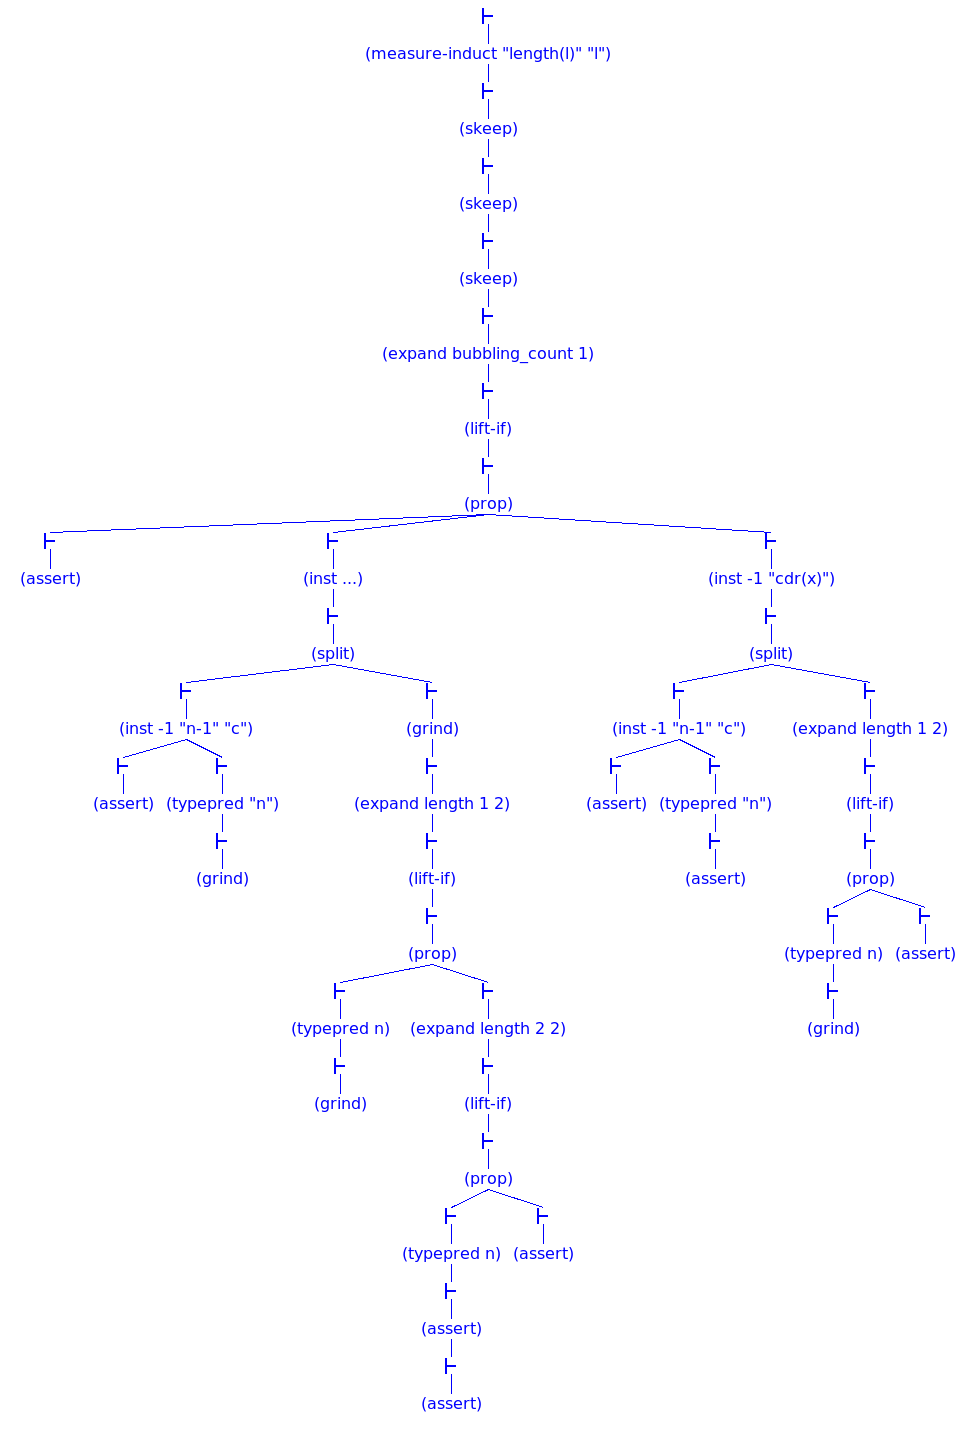
\includegraphics[width=0.75\linewidth,trim={8cm 20cm 4cm 10cm},clip]{figures/bubbling-counts-n.png}
    \caption{Casos da prova após a expansão da definição de \texttt{bubbling\_count}. O
    ramo omitido mais à esquerda é o caso base.}
    \label{fig:bubbling2}
\end{figure}


O restante da prova consiste em algumas instanciações adicionais de $c$ e/ou $n$, 
na expansão da definição de \texttt{length} e inferências sobre o tipo de $n$.
Felizmente existe a restrição de que $n < |l|$, e o comando \texttt{(typepred n)}
realiza essa inferência. O uso de \texttt{(grind)} após \texttt{(typepred n)}
foi basicamente um atalho para \texttt{(expand list2finseq)}
seguido de \texttt{(assert)}, ou de alguma resolução dos casos distintos
de \texttt{length}, que surge a partir da definição de \texttt{list2finseq}
(Figura \ref{fig:bubbling3}).

\begin{figure}[h!]
    \centering
    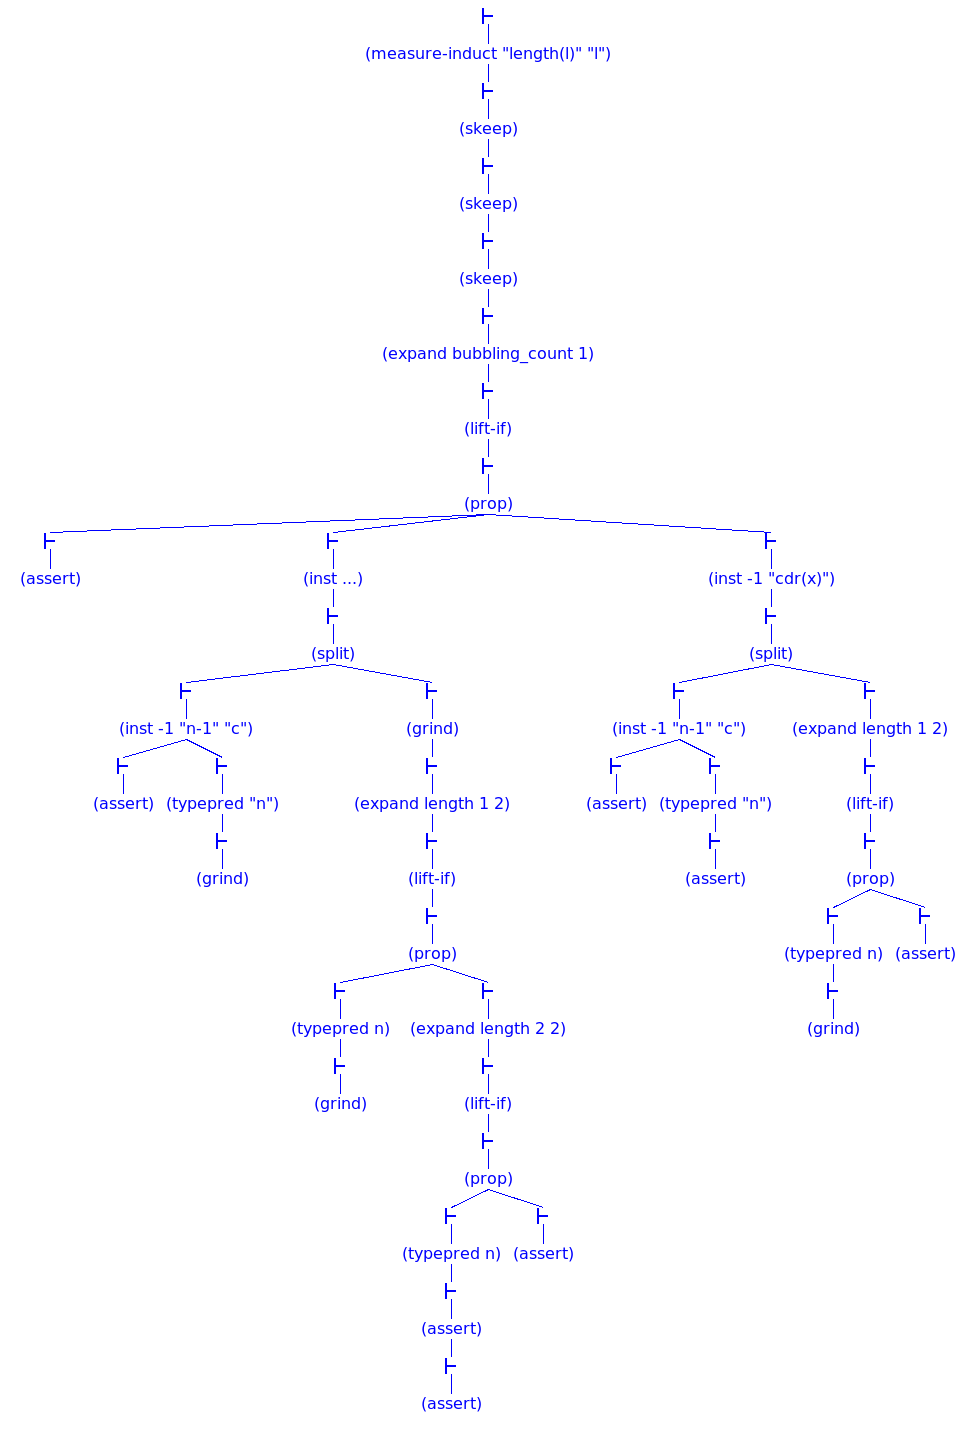
\includegraphics[width=0.25\linewidth,trim={20.5cm 10cm 0cm 18.5cm},clip]{figures/bubbling-counts-n.png}
    \caption{Para finalizar os ramos, foi necessário expandir a definição de
    \texttt{length} e realizar uma inferência sobre o tipo de $n$.}
    \label{fig:bubbling3}
\end{figure}


Dizemos então que \texttt{bubbling\_count} tem complexidade linear, $O(n)$.
Como $n<|l|$ por definição, então a função também é $O(|l|)$.
Resta então mostrar que o mesmo
se aplica a função original, \texttt{bubbling}, e isto foi feito mostrando que
\texttt{bubbling} e \texttt{bubbling\_count} são equivalentes:

\paragraph{Lema \ref{lemma:bequiv}: \texttt{bubbling\_equiv}:} 
\begin{equation*}
    \forall_{l,n,c} bubbling(l, n)_1 = bubbling\_count(l, c, n)_1 \hspace{1cm}, n<|l|, c\in \mathbb{N}
\end{equation*}

\paragraph{Estratégia da prova:} indução forte sobre $|l|$, pelo mesmo motivo
que no lema \ref{lemma:bcount} já que a prova se refere à mesma função,
\texttt{bubbling\_count}, que divide a lista da mesma forma que
\texttt{bubbling}. A diferença principal entre prova deste lema e a do lema
\ref{lemma:bcount} é que é necessário expandir as definições de ambas as
funções, \texttt{bubbling} e \texttt{bubbling\_count} antes de instanciar
a \HI. As instanciações da \HI foram realizdas como na prova do
lema \ref{lemma:bcount} (Figura \ref{fig:bubbling4}).

\begin{figure}[H]
    \centering
    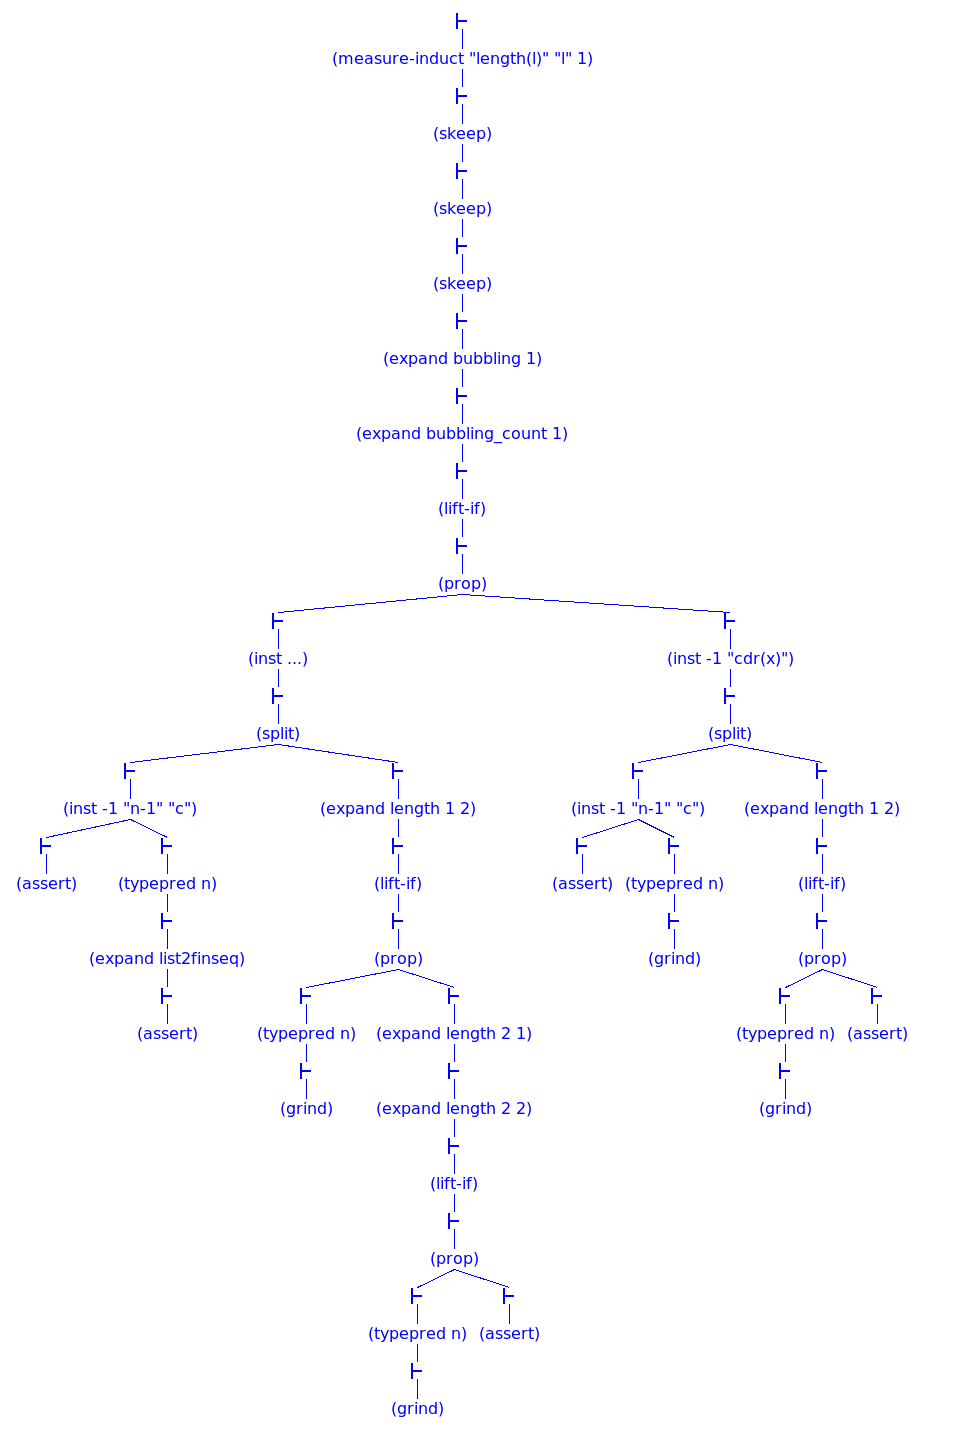
\includegraphics[width=0.\linewidth,trim={5cm 19cm 3cm 8cm},clip]{figures/bubbling-equiv.png}
    \caption{A prova do lema de equivalência entre \texttt{bubbling} e
    \texttt{bubbling\_count} requer a expansão de ambas as funções,
    mas segue de forma semelhante ao lema de complexidade.}
    \label{fig:bubbling4}
\end{figure}


\paragraph{Lema \ref{lemma:blen}: \texttt{bubbling\_length}:}
\begin{equation*}
    \forall_{l,n,c} |bubbling\_count(l, c, n)_1| = |l| \hspace{1cm}, n<|l|, c\in \mathbb{N}
\end{equation*}

\paragraph{Estratégia da prova:} indução forte sobre $|l|$, pelo mesmo motivo
que no lema \ref{lemma:bcount} já que a prova se refere à mesma função,
\texttt{bubbling\_count}. Este lema não está diretamente relacionado com
a analise da complexidade ou com a equivalência entre as funções. Contudo,
ele foi utilizado em alguns pontos das provas subsequentes e, por se tratar
de um lema relativamente longo de ser provado, decidimos enunciá-lo
separadamente. O objetivo deste lema é mostrar que \texttt{bubbling\_count}
retorna uma lista do mesmo tamanho que a lista de entrada, e a prova também
consiste em mostrar que isso é verdade para cada um dos casos da função
\texttt{bubbling\_count}.



\subsubsection{\textit{Bubblesort\_aux}}

\paragraph{Lema \ref{lemma:bacount}: \texttt{bubaux\_counts\_n2}:}
\begin{equation*}
    \forall_{l,n,c} bubblesort\_aux\_count(l, c, n)_2 = c + \frac{n^2 + n}{2} \hspace{1cm}, n<|l|, c\in \mathbb{N}
\end{equation*}

\paragraph{Estratégia da prova:} indução forte sobre $|l| + n$. A função
\texttt{bubblesort\_aux\_count} é uma função que faz chamadas
recursivas sobre $l$, e seria correspondente ao próprio Algoritmo
\ref{algo:bubblesort} menos as linhas 5 a 9 (que correspondem melhor com
a função \texttt{bubbling}). A principal questão aqui é que $|l|$
se mantém constante ao longo das chamadas de \texttt{bubblesort\_aux\_count},
portanto uma indução sobre $|l|$ não geraria uma \HI que pudesse ser
instanciada de maneira apropriada.
Uma segunda opção seria realizar a indução sobre $n$, uma vez que ele
é o parâmetro que varia ao longo das chamadas recursivas da função. No
entanto, como $n$ é dependente de $|l|$, foi necessário que a indução
fosse realizada sobre ambos os parâmetros simultaneamente,
daí a escolha de $|l| + n$:
\begin{lstlisting}
  |-------
{1}   FORALL (l: list[nat], n: below[list2finseq(l)`length]) (c: nat):
        bubblesort_aux_count(l, c, n)`2 = c + ((n ^ 2 + n) / 2)

Rule? (measure-induct "length(l) + n" ("l" "n"))
\end{lstlisting} 

A expansão da definição da definição de \texttt{bubbling\_count} após a escolha
da estratégia de prova, resulta em dois casos: o caso base em que
$n=0$ é trivial, pois consiste em provar que $c = c + \frac{n^2 + n}{2}$.
No segundo caso, precisamos provar o sequente:

\begin{lstlisting}
[-1]  (H.I.)
  |-------
{1}   x_2 = 0
{2}   bubblesort_aux_count(bubbling_count(x_1, c, x_2)`1,
                           bubbling_count(x_1, c, x_2)`2, x_2 - 1)`2
       = ((x_2 ^ 2 + x_2) / 2) + c

Rule? (inst -1 "bubbling_count(x_1, c, x_2)`1" "x_2-1")
\end{lstlisting} 

O que permite a instanciação da hipótese de indução da seguinte forma:

\begin{alignat*}{3}
bubblesort\_aux\_count(l, c, n)_2 &= c + ((n ^ 2 + n) / 2) && (h.i.)\\
l &= bubbling\_count(x_1, c, x_2)_1 \\
c &= c \\
n &= x_2-1
\end{alignat*}

A partir deste ponto, a prova novamente se ramifica em duas partes devido
a estratégias ser indução sobre $|l| + n$. No primeiro ramo, que decorre do
do parâmetro $n$, podemos chamar o lema \ref{lemma:bcount} para mostrar que
as chamadas de \texttt{bubbling\_count} incrementam $n$ de forma linear
(Figura \ref{fig:bubaux1}, ramo da esquerda). O segundo ramo decorre
consiste em garantir que estamos instanciando a \HI com valores
estritamente menores do que aqueles no consequente, e prova disso
utiliza o resultado do lema \ref{lemma:blen} que mostra que
$|bubbling\_count(l,c,n)| + n - 1 < |l| + n$, com os valores devidamente
instanciados (Figura \ref{fig:bubaux1}, ramo da direita).

\begin{figure}[H]
    \centering
    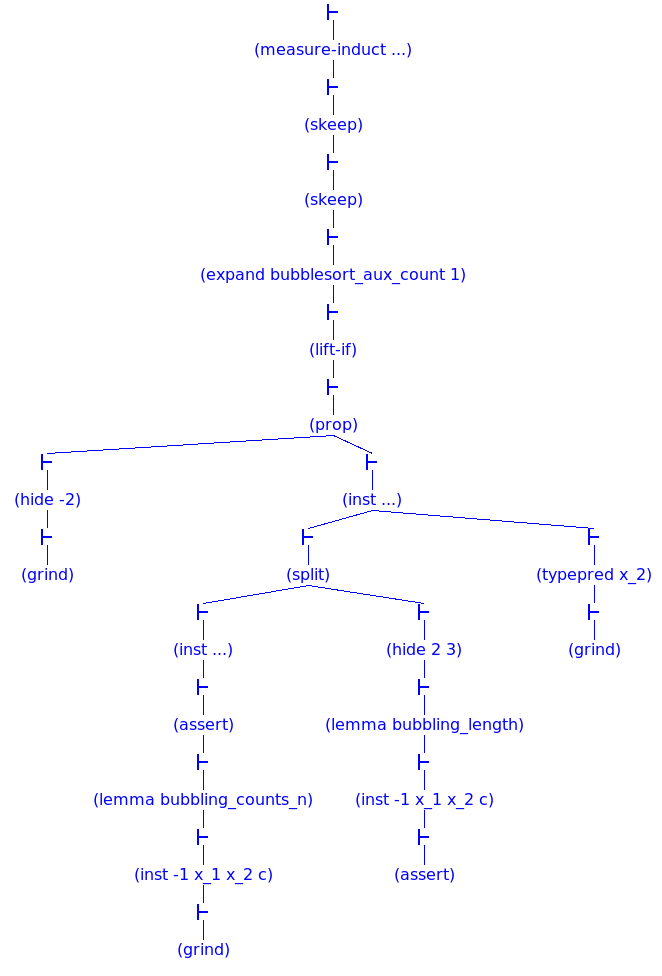
\includegraphics[width=0.75\linewidth,trim={2.5cm 0cm 3.5cm 12cm},clip]{figures/bubaux-counts-n2.png}
    \caption{Para finalizar análise da complexidade de
    \texttt{bubblesort\_aux} usamos os lemas \ref{lemma:bcount}
    e  \ref{lemma:blen} provados anteriormente. O ramo oculto
    ainda mais à direita se refere ao caso base.}
    \label{fig:bubaux1}
\end{figure}

Com isto, temos que a função \texttt{bubblesort\_aux\_count} realiza
$\frac{n^2 + n}{2}$ comparações e portanto é $O(n)$
Da mesma forma que com \texttt{bubbling}, pela restrição de $n<|l|$,
então também é $O(|l|)$. Aqui ainda precisamos mostrar a equivalência
entre os \texttt{bubblesort\_aux} com e sem contador, conforme realizado
a partir do lema a seguir.

\paragraph{Lema \ref{lemma:baequiv}: \texttt{bubblesort\_aux\_equiv}:}
\begin{equation*}
    \forall_{l,n,c} bubblesort\_aux(l, c, n)_1 = bubblesort\_aux\_count(l, c, n)_1    \hspace{1cm}, n<|l|, c\in \mathbb{N}
\end{equation*}

\paragraph{Estratégia da prova:} indução forte sobre $|l| + n$, pela mesma
razão que no lema \ref{lemma:bacount}, já também se refere à função
\texttt{bubblesort\_aux\_count} e \texttt{bubblesort\_aux} apresenta
as mesmas características.

A prova deste lema também requer a expansão da definição de ambas as
funções, \texttt{bubblesort\_aux\_count} e \texttt{bubblesort\_aux}.
Já que essas elas, chamam suas respectivas funções \texttt{bubbling},
podemos instanciar a \HI com a chamada interna de \texttt{bubbling}
de cada uma delas, e completar a prova a partir do lema \ref{lemma:bequiv}.
Da mesma forma que no lema de complexidade \ref{lemma:bacount}, esta
prova também precisa garantir que a instanciação da \HI foi realizada
de maneira adequada, o que também pode ser mostrado usando o resultado
do lema \ref{lemma:blen} sobre o tamanho de $l$ (Figura \ref{fig:bubaux2}).

\begin{figure}[H]
    \centering
    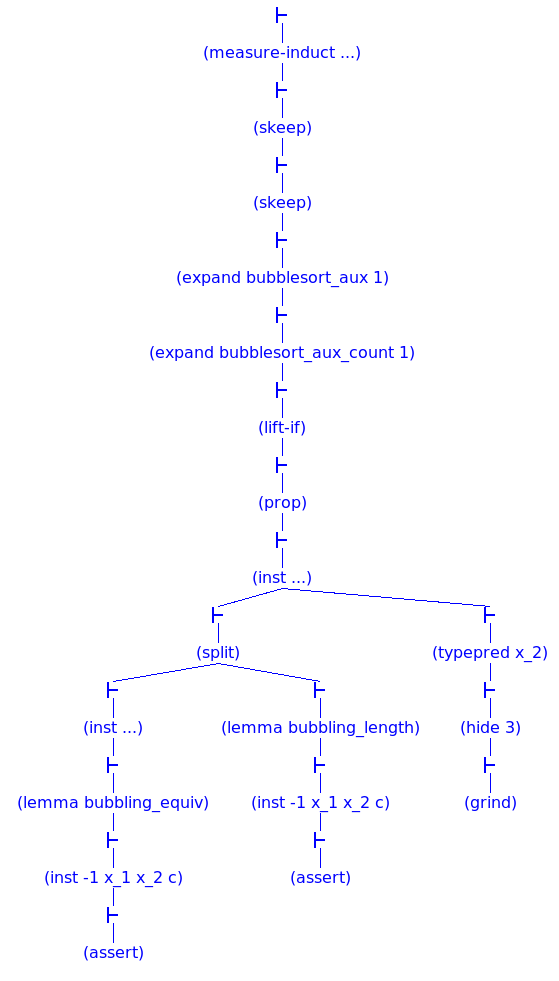
\includegraphics[width=0.75\linewidth,trim={0 0 3.5cm 14cm},clip]{figures/bubblesort-aux-equiv.png}
    \caption{Para finalizar análise de equivalência
    \texttt{bubblesort\_aux} entre \texttt{bubblesort\_aux\_count}
    usamos os lemas \ref{lemma:bequiv} e \ref{lemma:blen}
    provados anteriormente. O ramo oculto mais à direita se
    refere ao caso base.}
    \label{fig:bubaux2}
\end{figure}



\subsubsection{\textit{Bubblesort}}

\paragraph{Lema \ref{lemma:bscount}: \texttt{bubblesort\_counts\_n2}:}
\begin{equation*}
    \forall_{l} bubblesort\_count(l)_2 = \frac{|l|^2 - |l|}{2}
\end{equation*}

\paragraph{Estratégia da prova:} direta, a partir da aplicação do
lema \ref{lemma:bacount}. O objetivo da função \texttt{bubblesort\_count}
é encapsular \texttt{bubblesort\_aux\_count}, garantindo que esta
seja chamada com os parâmetros corretos. A prova deste lema consiste
na expansão da definição de \texttt{bubblesort\_count} após instanciar
$l$ para uma lista qualquer. Nos deparamos então com os dois casos
presentes na definição de \texttt{bubblesort\_count}: o primeiro caso,
em que a lista é vazia, é trivial, pois $\frac{|l|^2 - |l|}{2} = 0$.
No segundo caso, podemos evocar o lema \ref{lemma:bacount} e instanciá-lo
adequadamente pois sabemos exatamente os valores de $c$ e $n$ que serão
passados para \texttt{bubblesort\_aux\_count}, e como eles se
relacionam com $|l|$. O comando \texttt{(grind)} utilizado nos ramos
desta prova foram utilizados para realizar as expansões da definição de
\texttt{length} e fazer as simplificações algébricas apropriadas
(Figura \ref{fig:bsort1}).

\paragraph{Lema \ref{lemma:bsequv}: \texttt{bubblesort\_equiv}:}
\begin{equation*}
    \forall_{l} bubblesort(l)_1 = bubblesort\_count(l)_1 = \frac{|l|^2 - |l|}{2}
\end{equation*}

\paragraph{Estratégia da prova:} direta, a partir da aplicação do
lema \ref{lemma:baequiv}. De forma semelhante ao lema anterior, 
a prova foi feita a partir da aplicação do lema \ref{lemma:baequiv}.
A expansão das definições de ambas \texttt{bubblesort} e \texttt{bubblesort\_count}
revela a chamada das funções \texttt{bubblesort\_aux} e \texttt{bubblesort\_aux\_count}
e a igualdade é estabelecida por meio da instanciação do lema.
Novamente, o comando \texttt{(grind)} foi utilizado para fazer
as simplificações algébricas apropriadas e completar a prova
(Figura \ref{fig:bsort2}).

\begin{figure}[H]
\begin{minipage}{0.475\linewidth}
    \centering
    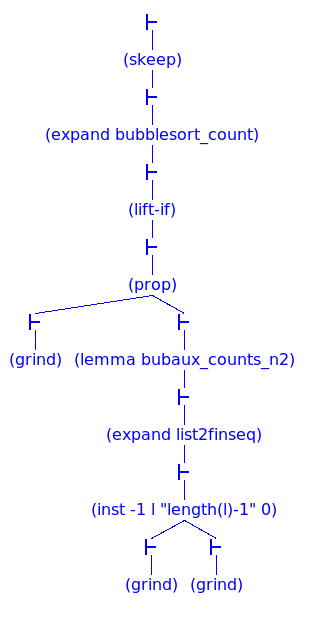
\includegraphics[width=\linewidth,trim={0 0 0 0},clip]{figures/bubblesort-count.png}
    \caption{A prova do lema de complexidade do \texttt{bubblesort\_count}
    é direta a partir da aplicação do lema \ref{lemma:bacount}, pois sabemos
    os valores exatos de $n$ e $c$, para uma dada lista $l$, que serão passados
    para \texttt{bubblesort\_aux}.}
    \label{fig:bsort1}
\end{minipage}
\hfill
\begin{minipage}{0.475\linewidth}
    \centering
    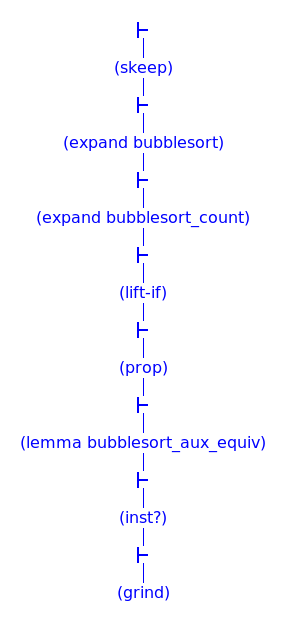
\includegraphics[width=\linewidth,
    trim={0 0 0 0},clip]{figures/bubblesort-equiv.png}
    \caption{A prova de equivalência entre \texttt{bubblesort} e
    \texttt{bubblesort\_count} é direta a partir da aplicação do
    lema \ref{lemma:baequiv}.}
    \label{fig:bsort2}
\end{minipage}
\end{figure}

\subsection{TCCs}

Ao final das provas dos lemas elaborados ainda restaram alguns TCCs 
(\textit{Type-Correctness Conditions}) que não puderam ser verificados
automaticamente pelo PVS. Isto foi parcialmente resolvido após uma mudança
na ordem em que os lemas foram enunciados no arquivo de entrada.
Faltou, contudo, realizar a prova de TCCs relacionados com a função
\texttt{bubbling}, e estes precisaram ser provados manualmente, pois necessitaram
de uma prova um pouco mais elaborada, embora ainda relativamente curta. A título
de exemplo, apresentaremos o \texttt{bubbling\_TCC3}, mas os
outros consistiam de sequentes semelhantes relacionados ao comprimento
de partes das listas.
\begin{lstlisting}
  |-------
{1}   FORALL (l: list[nat], (n: below[list2finseq[nat](l)`length])):
        car(l) > car(cdr(l)) AND NOT n = 0 IMPLIES
         n - 1 >= 0 AND n - 1 < list2finseq[nat]
               (cons[nat](car[nat](l), cdr[nat](cdr[nat](l))))`length
\end{lstlisting}

A prova deste sequente foi direta e se deu principalmente pela expansão
de \texttt{list2finseq}, e posteriormente a manipulação das definições
de \texttt{length} que surgiram (Figura \ref{fig:tcc}).


\begin{figure}[H]
\begin{minipage}{0.45\linewidth}
    \centering
    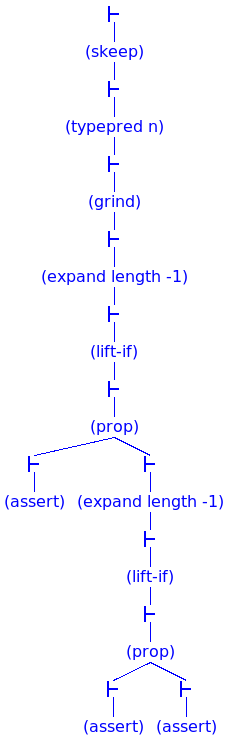
\includegraphics[height=0.4\textheight,width=0.8\linewidth,trim={0 9.7cm 0 0},clip]{figures/bubbling-tcc3.png}
\end{minipage}
\hfill
\begin{minipage}{0.45\linewidth}
    \centering
    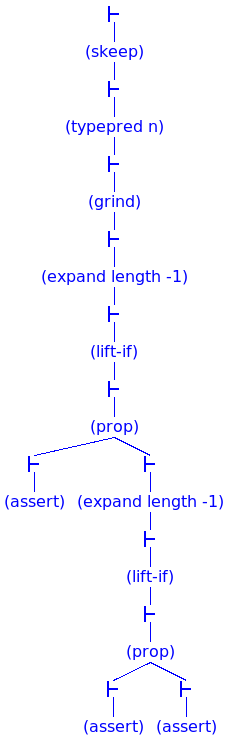
\includegraphics[height=0.4\textheight,width=0.8\linewidth,
    trim={0 0 0 9.7cm},clip]{figures/bubbling-tcc3.png}
\end{minipage}
    \caption{Prova do TCC \texttt{bubbling\_TCC3} que não pode ser completado
    automaticamente pelo PVS.}
    \label{fig:tcc}
\end{figure}



\section{Conclusão}
Neste trabalho, foi realizada uma prova assistida da complexidade quadrática do algoritmo de ordenação \textit{bubblesort} utilizando o PVS.
A prova foi realizada de forma indireta, mostrando que a contagem do número de trocas realizadas por uma implementação recursiva do algoritmo \textit{bubblesort} é igual a uma função quadrática do tamanho da lista de entrada.
Além disso, foi mostrado que a função \textit{bubblesort} é equivalente à sua versão com adição do contador do número de trocas. 
Portanto, concluímos que o algoritmo \textit{bubblesort} possui complexidade assintótica $O(n^2)$.


\clearpage

\bibliographystyle{unsrt}
\bibliography{bibliography}


\end{document}

%%% Local Variables:
%%% mode: latex
%%% TeX-master: t
%%% End:
